\documentclass{article}%
\usepackage[T1]{fontenc}%
\usepackage[utf8]{inputenc}%
\usepackage{lmodern}%
\usepackage{textcomp}%
\usepackage{lastpage}%
\usepackage{parskip}%
\usepackage[top=1.2in,bottom=1in,left=0.6in,right=0.6in,headsep=0.8in]{geometry}%
\usepackage{amsmath}%
\usepackage{graphicx}%
\usepackage{needspace}%
\usepackage{color}%
\usepackage{longtable}%
\usepackage{multirow}%
\usepackage[table]{xcolor}%
\usepackage{fancyhdr}%
\usepackage{tabularx}%
%
\definecolor{OsdagGreen}{HTML}{D5DF93}%
\fancypagestyle{header}{ 
\renewcommand{\headrulewidth}{0pt}%
\renewcommand{\footrulewidth}{0pt}%
\fancyhead{ 
}%
\fancyfoot{ 
}%
\fancyhead[C]{ 
\begin{tabularx}{\textwidth}{|l|p{6cm}|l|X|}%
\hline%
\rowcolor{OsdagGreen}%
Company Name&LoremIpsum&Project Title&Fossee\\%
\hline%
\rowcolor{OsdagGreen}%
Group/Team Name&LoremIpsum&Subtitle&\\%
\hline%
\rowcolor{OsdagGreen}%
Designer&LoremIpsum&Job Number&123\\%
\hline%
\rowcolor{OsdagGreen}%
Date&26 /05 /2020&Client&LoremIpsum\\%
\hline%
\end{tabularx}
}%
\fancyfoot[R]{ 
Page \thepage\ of \pageref{LastPage}
}
}%
%
\begin{document}%
\normalsize%
\pagestyle{header}%
\section{Input Parameters}%
\label{sec:InputParameters}%
\renewcommand{\arraystretch}{1.2}%
\begin{longtable}{|p{5cm}|p{2cm}|p{2cm}|p{2cm}|p{5cm}|}%
\hline%
\hline%
\multicolumn{3}{|c|}{Module}&\multicolumn{2}{|c|}{Beam Coverplate Connection}\\%
\hline%
\hline%
\multicolumn{3}{|c|}{MainModule}&\multicolumn{2}{|c|}{Moment Connection}\\%
\hline%
\hline%
\multicolumn{3}{|c|}{Moment(kNm)*}&\multicolumn{2}{|c|}{5.0}\\%
\hline%
\hline%
\multicolumn{3}{|c|}{Shear (kN)*}&\multicolumn{2}{|c|}{62.0}\\%
\hline%
\hline%
\multicolumn{3}{|c|}{Axial (kN) *}&\multicolumn{2}{|c|}{151.0}\\%
\hline%
\hline%
\multicolumn{5}{|c|}{\textbf{Section}}\\%
\hline%
\hline%
\multirow{12}{*}{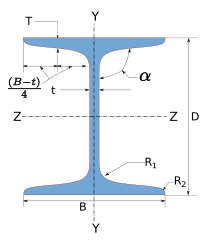
\includegraphics[width=5cm,height=5cm]{E:/office _anjali/columnspliceanjali/Osdag3/ResourceFiles/images/ISection.png}}&\multicolumn{2}{|c|}{Beam Section *}&\multicolumn{2}{|c|}{MB 450}\\%
\cline{2%
-%
5}%
&\multicolumn{2}{|c|}{Preferences}&\multicolumn{2}{|c|}{Outside + Inside}\\%
\cline{2%
-%
5}%
&\multicolumn{2}{|c|}{Material *}&\multicolumn{2}{|c|}{E 250 (Fe 410 W)A}\\%
\cline{2%
-%
5}%
&\multicolumn{2}{|c|}{Ultimate strength, fu (MPa)}&\multicolumn{2}{|c|}{410}\\%
\cline{2%
-%
5}%
&Yield Strength , fy (MPa)&250&R1(mm)&15.0\\%
\cline{2%
-%
5}%
&Mass&72.4&R2(mm)&7.5\\%
\cline{2%
-%
5}%
&Area(mm2) {-} A&9220.0&Iz(mm4)&303580000.0\\%
\cline{2%
-%
5}%
&D(mm)&450.0&Iy(mm4)&8070000.0\\%
\cline{2%
-%
5}%
&B(mm)&150.0&rz(mm)&181.0\\%
\cline{2%
-%
5}%
&t(mm)&9.4&ry(mm)&30.0\\%
\cline{2%
-%
5}%
&T(mm)&17.4&Zz(mm3)&1349300.0\\%
\cline{2%
-%
5}%
&FlangeSlope&98&Zy(mm3)&108000.0\\%
\cline{2%
-%
5}%
\hline%
\multicolumn{5}{|c|}{\textbf{Bolt Details}}\\%
\hline%
\hline%
\multicolumn{3}{|c|}{Diameter (mm)*}&\multicolumn{2}{|c|}{{[}12.0, 16.0, 20.0, 24.0, 30.0, 36.0{]}}\\%
\hline%
\hline%
\multicolumn{3}{|c|}{Grade *}&\multicolumn{2}{|c|}{{[}3.6, 4.6, 4.8, 5.6, 5.8, 6.8, 8.8, 9.8, 10.9, 12.9{]}}\\%
\hline%
\hline%
\multicolumn{3}{|c|}{Type *}&\multicolumn{2}{|c|}{Friction Grip Bolt}\\%
\hline%
\hline%
\multicolumn{3}{|c|}{Bolt hole type}&\multicolumn{2}{|c|}{Standard}\\%
\hline%
\hline%
\multicolumn{3}{|c|}{Slip factor (µ\_f)}&\multicolumn{2}{|c|}{0.3}\\%
\hline%
\hline%
\multicolumn{3}{|c|}{Type of edges}&\multicolumn{2}{|c|}{a {-} Sheared or hand flame cut}\\%
\hline%
\hline%
\multicolumn{3}{|c|}{Gap between beam and <br>support (mm)}&\multicolumn{2}{|c|}{10.0}\\%
\hline%
\hline%
\multicolumn{3}{|c|}{Are the members exposed to <br>corrosive influences}&\multicolumn{2}{|c|}{False}\\%
\hline%
\end{longtable}

%
\Needspace{10\baselineskip}%
\newpage%
\section{Design Checks}%
\label{sec:DesignChecks}%
\subsection{Member Capacity}%
\label{subsec:MemberCapacity}%
\renewcommand{\arraystretch}{1.2}%
\begin{longtable}{|p{4cm}|p{5cm}|p{5.5cm}|p{1.5cm}|}%
\hline%
\rowcolor{OsdagGreen}%
Check&Required&Provided&Remarks\\%
\hline%
\endhead%
\hline%
Axial Capacity Member Ac (kN)&&$\begin{aligned} A_c &=\frac{A*f_y}{\gamma_{m0} *10^3}\\ &=\frac{9220.0*250}{1.1* 10^3}\\ &=2095.45\end{aligned}$&\\%
\hline%
Shear Capacity Member Sc (kN)&&$\begin{aligned} S_c &= \frac{A_v*f_y}{\sqrt{3}*\gamma_{mo} *10^3}\\ &=\frac{415.2*9.4*250}{\sqrt{3}*1.1 *10^3}\\ &=512.12\end{aligned}$&\\%
\hline%
Plastic Moment Capacity Pmc (kNm)&&$\begin{aligned} Pmc &= \frac{\beta_b * Z_p *fy}{\gamma_{mo} * 10^6}\\ &=\frac{1*405118.94*250}{1.1 * 10^6}\\ &=92.07\end{aligned}$&\\%
\hline%
Moment Deformation Criteria Mdc (kNm)&&$\begin{aligned} Mdc &= \frac{1.5 *Z_e *fy}{1.1* 10^6}\\ &= \frac{1.5 *1349300.0*250}{1.1* 10^6}\\ &= 459.99\end{aligned}$&\\%
\hline%
Moment Capacity Member Mc (kNm)&&$\begin{aligned} M_c &= min(Pmc,Mdc)\\ &=min(92.07,459.99)\\ &=92.07\end{aligned}$&\\%
\hline%
\end{longtable}

%
\newpage%
\subsection{Load Consideration}%
\label{subsec:LoadConsideration}%
\renewcommand{\arraystretch}{1.2}%
\begin{longtable}{|p{4cm}|p{3.5cm}|p{6.5cm}|p{1.5cm}|}%
\hline%
\rowcolor{OsdagGreen}%
Check&Required&Provided&Remarks\\%
\hline%
\endhead%
\hline%
Applied Axial Load Au (kN)&$\begin{aligned} Ac_{min} &= 0.3 * A_c\\ &= 0.3 *2095.45\\ &=628.64\\ Ac_{max} &= Ac \\ &=2095.45\end{aligned}$&$\begin{aligned} A_u &=628.64\end{aligned}$&Pass\\%
\hline%
Applied Shear Load Vu (kN)&$\begin{aligned} Vc_{min} &= 0.6 * S_c\\ &= 0.6 *512.12\\ &=307.27\\ Vc_{max} &= Sc \\ &=512.12\end{aligned}$&$\begin{aligned} V_u &=307.27\end{aligned}$&Pass\\%
\hline%
Applied Moment Load Mu (kNm)&$\begin{aligned} Mc_{min} &= 0.5 * M_c\\ &= 0.5 *92.07\\ &=46.04\\  Mc_{max} &= Mc \\ &=92.07\end{aligned}$&$\begin{aligned} M_u &=46.04\end{aligned}$&Pass\\%
\hline%
Forces Carried by Web&&$\begin{aligned}A_w &= Axial~ force~ in~ web  \\   &= \frac{(D- 2*T)*t* Au }{A} \\ &= \frac{(450.0- 2*17.4)*9.4*628.64 }{9220.0} \\ &=266.11~ kN\\ M_w &= Moment ~in ~web  \\  &= \frac{Z_w * Mu}{Z} \\ &= \frac{405118.94 * 46.04}{1551600.0} \\ &=12.02~{kNm}\end{aligned}$&\\%
\hline%
Forces Carried by Flange&&$\begin{aligned} A_f&= Axial~force~ in ~flange  \\ &= \frac{Au * B *T}{A} \\ &= \frac{628.64 * 150.0*17.4}{9220.0} \\ &=177.95~ kN\\ M_f& =Moment~ in~ flange \\  & = Mu-M_w\\ &= 46.04-12.02\\ &=34.02~{kNm}\\  F_f& =flange~force  \\ & = \frac{M_f *10^3}{D-T} + A_f \\ &= \frac{34.02* 10^3}{450.0-17.4} +177.95 \\ &=256.59~kN \end{aligned}$&\\%
\hline%
\end{longtable}

%
\newpage%
\subsection{Initial Member Check}%
\label{subsec:InitialMemberCheck}%
\renewcommand{\arraystretch}{1.2}%
\begin{longtable}{|p{3cm}|p{4.5cm}|p{6.5cm}|p{1.5cm}|}%
\hline%
\rowcolor{OsdagGreen}%
Check&Required&Provided&Remarks\\%
\hline%
\endhead%
\hline%
Flange Tension Yielding Capacity (kN)&$\begin{aligned} F_f &=256.59\end{aligned}$&$\begin{aligned} T_{dg} &= \frac{l*t*f_y}{\gamma_{mo}}\\ &=\frac{1*150.0*17.4*250}{1.1}\\ &=593.18\end{aligned}$&Pass\\%
\hline%
Web Tension Yielding Capacity (kN)&$\begin{aligned} A_w &=266.11\end{aligned}$&$\begin{aligned} T_{dg} &= \frac{l*t*f_y}{\gamma_{mo}}\\ &=\frac{1*415.2*9.4*250}{1.1}\\ &=887\end{aligned}$&Pass\\%
\hline%
\end{longtable}

%
\newpage%
\subsection{Initial flange plate height check}%
\label{subsec:Initialflangeplateheightcheck}%
\renewcommand{\arraystretch}{1.2}%
\begin{longtable}{|p{4.5cm}|p{2.5cm}|p{7cm}|p{1.5cm}|}%
\hline%
\rowcolor{OsdagGreen}%
Check&Required&Provided&Remarks\\%
\hline%
\endhead%
\hline%
flange\_plate.Height&Outer.b >= 50&$\begin{aligned} Outer.b &=150.0\end{aligned}$&Pass\\%
\hline%
flange\_plate.InnerHeight&Inner.b >= 50&$\begin{aligned} inner.b &= \frac{B-t-(2*r_1)}{2}\\ &=\frac{150.0-9.4-(2*15.0)}{2}\\ &= 55.3\end{aligned}$&Pass\\%
\hline%
\end{longtable}

%
\newpage%
\subsection{Flange plate thickness}%
\label{subsec:Flangeplatethickness}%
\renewcommand{\arraystretch}{1.2}%
\begin{longtable}{|p{2.5cm}|p{4.5cm}|p{7cm}|p{1.5cm}|}%
\hline%
\rowcolor{OsdagGreen}%
Check&Required&Provided&Remarks\\%
\hline%
\endhead%
\hline%
Thickness (mm)*&$\begin{aligned} T &=8.7\end{aligned}$&$\begin{aligned} t_f &=12.0\end{aligned}$&Pass\\%
\hline%
Plate Area check (mm2)&$\begin{aligned} &pt.area >= \\&connected~member~area * 1.05\\  &= 2740.5\end{aligned}$&$\begin{aligned} outer.b &= B\\ &= 150.0 \\ inner.b &= \frac{B-t-(2*r_1)}{2}\\ &=\frac{150.0-9.4-(2*15.0)}{2}\\ &= 55.3 \\  pt.area &=(150.0+(2*55.3))*12.0\\ &= 3127.2\end{aligned}$&Pass\\%
\hline%
\end{longtable}

%
\newpage%
\subsection{Web plate thickness}%
\label{subsec:Webplatethickness}%
\renewcommand{\arraystretch}{1.2}%
\begin{longtable}{|p{2.5cm}|p{4.5cm}|p{7cm}|p{1.5cm}|}%
\hline%
\rowcolor{OsdagGreen}%
Check&Required&Provided&Remarks\\%
\hline%
\endhead%
\hline%
Thickness (mm)*&$\begin{aligned} t &=4.7\end{aligned}$&$\begin{aligned} t_w &=6.0\end{aligned}$&Pass\\%
\hline%
Plate Area check (mm2)&$\begin{aligned} &pt.area >= \\&connected~member~area * 1.05\\  &= 3604.52\end{aligned}$&$\begin{aligned} web~b &= D-(2*T)-(2*r_1)\\ &=450.0-(2*17.4)-(2*15.0)\\ &= 365.2 \\  pt.area &= 6.0*2* 365.2\\ &= 4382.4\end{aligned}$&Pass\\%
\hline%
\end{longtable}

%
\newpage%
\subsection{Web Spacing Checks}%
\label{subsec:WebSpacingChecks}%
\renewcommand{\arraystretch}{1.2}%
\begin{longtable}{|p{2.5cm}|p{7.5cm}|p{5cm}|p{1cm}|}%
\hline%
\rowcolor{OsdagGreen}%
Check&Required&Provided&Remarks\\%
\hline%
\endhead%
\hline%
Min.Diameter (mm)&&$\begin{aligned} d &=12.0\end{aligned}$&\\%
\hline%
Min. Gauge (mm)&$\begin{aligned}p/g_{min}&= 2.5 ~ d&\\ =&2.5*12.0&=30.0\end{aligned}$&$\begin{aligned} g &=30~(Row~Limit~(r_l) = 2)\end{aligned}$&\\%
\hline%
Min. Edge Distance (mm)&$\begin{aligned}e/e`_{min} &=[1.5~or~ 1.7] * d_0\\ &=1.7*13.0=22.1 \end{aligned}$&25&\\%
\hline%
Spacing Check&$\begin{aligned} depth & = 2 * e + (r_l -1) * g\\ & = 2 * 25+(2.0-1)*30\\ & = 80.0\end{aligned}$&365.2&Pass\\%
\hline%
\end{longtable}

%
\newpage%
\subsection{Flange Spacing Checks}%
\label{subsec:FlangeSpacingChecks}%
\renewcommand{\arraystretch}{1.2}%
\begin{longtable}{|p{2.5cm}|p{7.5cm}|p{5cm}|p{1cm}|}%
\hline%
\rowcolor{OsdagGreen}%
Check&Required&Provided&Remarks\\%
\hline%
\endhead%
\hline%
Min.Diameter (mm)&&$\begin{aligned} d &=12.0\end{aligned}$&\\%
\hline%
Min. Gauge (mm)&$\begin{aligned}p/g_{min}&= 2.5 ~ d&\\ =&2.5*12.0&=30.0\end{aligned}$&$\begin{aligned} g &=0.0~(Row~Limit~(r_l) = 1)\end{aligned}$&\\%
\hline%
Min. Edge Distance (mm)&$\begin{aligned}e/e`_{min} &=[1.5~or~ 1.7] * d_0\\ &=1.7*13.0=22.1 \end{aligned}$&25&\\%
\hline%
Spacing Check&$\begin{aligned} depth & = 2 * e + (r_l -1) * g\\ & = 2 * 25+(1.0-1)*30\\ & = 50.0\end{aligned}$&55.3&Pass\\%
\hline%
\end{longtable}

%
\newpage%
\subsection{Flange Bolt Checks}%
\label{subsec:FlangeBoltChecks}%
\renewcommand{\arraystretch}{1.2}%
\begin{longtable}{|p{4cm}|p{5cm}|p{5.5cm}|p{1.5cm}|}%
\hline%
\rowcolor{OsdagGreen}%
Check&Required&Provided&Remarks\\%
\hline%
\endhead%
\hline%
Diameter (mm)&Bolt Quantity Optimisation&$\begin{aligned} d &=12.0\end{aligned}$&\\%
\hline%
Grade&Bolt Grade Optimisation&12.9&\\%
\hline%
Bolt.fu&&1200.0&\\%
\hline%
Bolt.fy&&1080.0&\\%
\hline%
Hole Diameter (mm)& &$\begin{aligned} d_0 &=13.0\end{aligned}$&\\%
\hline%
Slip Resistance&&$\begin{aligned}V_{dsf} & = \frac{\mu_f~ n_e~  K_h~ F_o}{\gamma_{mf}}\\ & Where, F_o = 0.7 * f_{ub} A_{nb}\\ V_{dsf} & = \frac{0.3*1*1.0* 0.7 *1200.0*0.0}{1.25}\\ & =33.99\end{aligned}$&\\%
\hline%
No of Bolts&$\begin{aligned}R_{u} &= \sqrt{V_u^2+A_u^2}\\ n_{trial} &= R_u/ V_{bolt}\\ R_{u} &= \frac{\sqrt{0.0^2+256.59^2}}{33.99}\\ &=16\end{aligned}$&16&\\%
\hline%
No of Columns&&$\begin{aligned} n_c &=8\end{aligned}$&\\%
\hline%
No of Rows&&$\begin{aligned} n_r &=2\end{aligned}$&\\%
\hline%
Min. Pitch (mm)&$\begin{aligned}p/g_{min}&= 2.5 ~ d&\\ =&2.5*12.0&=30.0\end{aligned}$&30&Pass\\%
\hline%
Max. Pitch (mm)&$\begin{aligned}p/g_{max} &=\min(32~t,~300~mm)&\\ &=\min(32 *~12.0,~ 300 ~mm)\\&=300\end{aligned}$&30&Pass\\%
\hline%
Min. Gauge (mm)&$\begin{aligned}p/g_{min}&= 2.5 ~ d&\\ =&2.5*12.0&=30.0\end{aligned}$&0.0&N/A\\%
\hline%
Max. Gauge (mm)&$\begin{aligned}p/g_{max} &=\min(32~t,~300~mm)&\\ &=\min(32 *~12.0,~ 300 ~mm)\\&=300\end{aligned}$&0.0&N/A\\%
\hline%
Min. End Distance (mm)&$\begin{aligned}e/e`_{min} &=[1.5~or~ 1.7] * d_0\\ &=1.7*13.0=22.1 \end{aligned}$&25&Pass\\%
\hline%
Max. End Distance (mm)&$\begin{aligned}e/e`_{max} &= 12~ t~ \varepsilon&\\ \varepsilon &= \sqrt{\frac{250}{f_y}}\\ e/e`_{max}&=12 ~*12.0*\sqrt{\frac{250}{250}}\\ &=144.0\\ \end{aligned}$&25&Pass\\%
\hline%
Min. Edge Distance (mm)&$\begin{aligned}e/e`_{min} &=[1.5~or~ 1.7] * d_0\\ &=1.7*13.0=22.1 \end{aligned}$&27.65&Pass\\%
\hline%
Max. Edge Distance (mm)&$\begin{aligned}e/e`_{max} &= 12~ t~ \varepsilon&\\ \varepsilon &= \sqrt{\frac{250}{f_y}}\\ e/e`_{max}&=12 ~*12.0*\sqrt{\frac{250}{250}}\\ &=144.0\\ \end{aligned}$&27.65&Pass\\%
\hline%
Bolt Capacity post Long Joint (kN)&$\begin{aligned} &if~l\geq 15 * d~then~V_{rd} = \beta_{ij} * V_{db} \\ & if~l < 15 * d~then~V_{rd} = V_{db} \\ & where,\\ & l = ((nc~or~nr) - 1) * (p~or~g) \\ & \beta_{ij} = 1.075 - l/(200 * d) \\ & but~0.75\leq\beta_{ij}\leq1.0 \end{aligned}$&$\begin{aligned} l~&= ((nc~or~nr) - 1) * (p~or~g) \\  lc&= 2*((\frac{8}{2} - 1) * 30+25)+ 10.0\\&=240.0\\  lr&= 2*((\frac{2}{2} - 1) * 0.0+27.65\\& +15.0)+ 9.4=94.7\\  l~&= 240.0\\ &15 * d = 15 * 12.0 = 180.0 \\ &since,~l \geq 15 * d~\\ &then~V_{rd} = \beta_{ij} * V_{db} \\ \beta_{ij} &= 1.075 - 240.0/(200*12.0)\\& =0.98\\  V_{rd}& = 0.98 * 33.99=33.31 \end{aligned}$&\\%
\hline%
Capacity (kN)&32.07&33.31&Pass\\%
\hline%
\end{longtable}

%
\newpage%
\subsection{Web Bolt Checks}%
\label{subsec:WebBoltChecks}%
\renewcommand{\arraystretch}{1.2}%
\begin{longtable}{|p{4cm}|p{5cm}|p{5.5cm}|p{1.5cm}|}%
\hline%
\rowcolor{OsdagGreen}%
Check&Required&Provided&Remarks\\%
\hline%
\endhead%
\hline%
Slip Resistance&&$\begin{aligned}V_{dsf} & = \frac{\mu_f~ n_e~  K_h~ F_o}{\gamma_{mf}}\\ & Where, F_o = 0.7 * f_{ub} A_{nb}\\ V_{dsf} & = \frac{0.3*1*1.0* 0.7 *1200.0*84.3}{1.25}\\ & =33.99\end{aligned}$&\\%
\hline%
No of Bolts&$\begin{aligned}R_{u} &= \sqrt{V_u^2+A_u^2}\\ n_{trial} &= R_u/ V_{bolt}\\ R_{u} &= \frac{\sqrt{307.27^2+266.11^2}}{33.99}\\ &=24\end{aligned}$&60&\\%
\hline%
No of Columns&&$\begin{aligned} n_c &=6\end{aligned}$&\\%
\hline%
No of Rows&&$\begin{aligned} n_r &=10\end{aligned}$&\\%
\hline%
Min. Pitch (mm)&$\begin{aligned}p/g_{min}&= 2.5 ~ d&\\ =&2.5*12.0&=30.0\end{aligned}$&30&Pass\\%
\hline%
Max. Pitch (mm)&$\begin{aligned}p/g_{max} &=\min(32~t,~300~mm)&\\ &=\min(32 *~6.0,~ 300 ~mm)\\&=192.0\end{aligned}$&30&Pass\\%
\hline%
Min. Gauge (mm)&$\begin{aligned}p/g_{min}&= 2.5 ~ d&\\ =&2.5*12.0&=30.0\end{aligned}$&30&Pass\\%
\hline%
Max. Gauge (mm)&$\begin{aligned}p/g_{max} &=\min(32~t,~300~mm)&\\ &=\min(32 *~6.0,~ 300 ~mm)\\&=192.0\end{aligned}$&30&Pass\\%
\hline%
Min. End Distance (mm)&$\begin{aligned}e/e`_{min} &=[1.5~or~ 1.7] * d_0\\ &=1.7*13.0=22.1 \end{aligned}$&25&Pass\\%
\hline%
Max. End Distance (mm)&$\begin{aligned}e/e`_{max} &= 12~ t~ \varepsilon&\\ \varepsilon &= \sqrt{\frac{250}{f_y}}\\ e/e`_{max}&=12 ~*6.0*\sqrt{\frac{250}{250}}\\ &=72.0\\ \end{aligned}$&25&Pass\\%
\hline%
Min. Edge Distance (mm)&$\begin{aligned}e/e`_{min} &=[1.5~or~ 1.7] * d_0\\ &=1.7*13.0=22.1 \end{aligned}$&25&Pass\\%
\hline%
Max. Edge Distance (mm)&$\begin{aligned}e/e`_{max} &= 12~ t~ \varepsilon&\\ \varepsilon &= \sqrt{\frac{250}{f_y}}\\ e/e`_{max}&=12 ~*6.0*\sqrt{\frac{250}{250}}\\ &=72.0\\ \end{aligned}$&25&Pass\\%
\hline%
Parameters required for bolt force (mm)&&$\begin{aligned} l_n~~~ &= length~available \\  l_n~~~ &= (n_r - 1) * g\\  &= (10 - 1) *30\\  & =270\\  y_{max} &= l_n / 2\\  &= 270 / 2 \\  & =135.0\\ x_{max} &= p * (\frac{n_c}{2} - 1) / 2 \\  &= 30 * (\frac{6}{2} + - 1) / 2 \\  & =30.0\end{aligned}$&\\%
\hline%
Moment Demand (kNm&&$\begin{aligned}  M_d &= (V_u * ecc + M_w)\\  &= \frac{(307.27 * 10^3 *75.0 + 12.02*10^6)}{10^6}\\  & =35.07\end{aligned}$&\\%
\hline%
Bolt.Force&&$\begin{aligned} vbv~~ &= V_u / (n_r * n_c)\\  &= \frac{307.27}{ (10*6)}\\  & =10.24\\ tmh~ &= \frac{M_d * y_{max} }{ \Sigma r_i^2} \\  &= \frac{35.07 *135.0}{240.75}\\  & =19.66\\  tmv ~&= \frac{M_d * x_{max}}{\Sigma r_i^2}\\ &= \frac{35.07 * 30.0}{240.75}\\  & =4.37\\  abh~ & = \frac{A_u }{(n_r * n_c)}\\   & =\frac{266.11}{ (10 *6)}\\  & =8.87\\  vres &=\sqrt{(vbv +tmv) ^ 2 + (tmh+abh) ^ 2}\\   &= \sqrt{(10.24 +4.37) ^2 + (19.66+8.87) ^ 2}\\  & =32.06\end{aligned}$&\\%
\hline%
Bolt Capacity post Long Joint (kN)&$\begin{aligned} &if~l\geq 15 * d~then~V_{rd} = \beta_{ij} * V_{db} \\ & if~l < 15 * d~then~V_{rd} = V_{db} \\ & where,\\ & l = ((nc~or~nr) - 1) * (p~or~g) \\ & \beta_{ij} = 1.075 - l/(200 * d) \\ & but~0.75\leq\beta_{ij}\leq1.0 \end{aligned}$&$\begin{aligned} l&= ((nc~or~nr) - 1) * (p~or~g) \\  lc&= 2*((\frac{6}{2} - 1) * 30+25)+ 10.0\\&=180.0\\  lr&= (10 - 1) * 30=270\\  l&= 270\\ & 15 * d = 15 * 12.0 = 180.0 \\ &since,~l \geq 15 * d~ \\&then~V_{rd} = \beta_{ij} * V_{db} \\ \beta_{ij} &= 1.075 - 270/(200*12.0) \\&=0.96\\ V_{rd} &= 0.96 * 33.99=32.63 \end{aligned}$&\\%
\hline%
Capacity (kN)&32.06&32.63&Pass\\%
\hline%
\end{longtable}

%
\newpage%
\subsection{Inner and Outer flange plate Checks}%
\label{subsec:InnerandOuterflangeplateChecks}%
\renewcommand{\arraystretch}{1.2}%
\begin{longtable}{|p{4cm}|p{6cm}|p{5.5cm}|p{1.5cm}|}%
\hline%
\rowcolor{OsdagGreen}%
Check&Required&Provided&Remarks\\%
\hline%
\endhead%
\hline%
Min. Plate Height (mm)&$\begin{aligned}min~flange~plate~ht &= beam~width\\ &=150.0\end{aligned}$&150.0&Pass\\%
\hline%
Min. Plate Length (mm)&$\begin{aligned} & 2[2*e_{min} + ({\frac{bolt~lines}{2}}-1) * p_{min})]\\ & +\frac{gap}{2}]\\ &=2*[(2*22.1 + (\frac{8}{2}-1) * 30.0\\ &= + \frac{10.0}{2}]\\ &=278.4\end{aligned}$&290.0&Pass\\%
\hline%
Min. Inner Plate Height (mm)&$\begin{aligned}&= \frac{B -t- (2*R1)}{2}\\ &=\frac{150.0 -9.4 - 2*15.0}{2}\\ &=55.3\end{aligned}$&55.3&Pass\\%
\hline%
Max. Inner Plate Height (mm)&$\begin{aligned}&= \frac{B -t- (2*R1)}{2}\\ &=\frac{150.0 -9.4 - 2*15.0}{2}\\ &=55.3\end{aligned}$&55.3&Pass\\%
\hline%
Min. Inner Plate Length (mm)&$\begin{aligned} & 2[2*e_{min} + ({\frac{bolt~lines}{2}}-1) * p_{min})]\\ & +\frac{gap}{2}]\\ &=2*[(2*22.1 + (\frac{8}{2}-1) * 30.0\\ &= + \frac{10.0}{2}]\\ &=278.4\end{aligned}$&290.0&Pass\\%
\hline%
Min.Plate Thickness (mm)&$\begin{aligned} t_w=8.7\end{aligned}$&12.0&Pass\\%
\hline%
\end{longtable}

%
\newpage%
\subsection{Member Checks}%
\label{subsec:MemberChecks}%
\renewcommand{\arraystretch}{1.2}%
\begin{longtable}{|p{4cm}|p{6cm}|p{5.5cm}|p{1.5cm}|}%
\hline%
\rowcolor{OsdagGreen}%
Check&Required&Provided&Remarks\\%
\hline%
\endhead%
\hline%
Flange Tension Yielding Capacity (kN)&&$\begin{aligned} T_{dg} &= \frac{l*t*f_y}{\gamma_{mo}}\\ &=\frac{1*150.0*17.4*250}{1.1}\\ &=593.18\end{aligned}$&\\%
\hline%
Flange Tension Rupture Capacity (kN)&&$\begin{aligned} T_{dn} &= \frac{0.9*A_{n}*f_u}{\gamma_{m1}}\\ &=\frac{0.9*(150.0-2*13.0)*17.4*410}{1.25}\\ &=636.92\end{aligned}$&\\%
\hline%
Flange Block Shear Capacity (kN)&&$\begin{aligned}T_{db1} &= \frac{A_{vg} f_{y}}{\sqrt{3} \gamma_{m0}} + \frac{0.9 A_{tn} f_{u}}{\gamma_{m1}}\\ T_{db2} &= \frac{0.9*A_{vn} f_{u}}{\sqrt{3} \gamma_{m1}} + \frac{A_{tg} f_{y}}{\gamma_{m0}}\\ T_{db} &= min(T_{db1}, T_{db2})= 630.9\end{aligned}$&\\%
\hline%
Flange Tension Capacity (kN)&$\begin{aligned} f_f &=256.59\end{aligned}$&$\begin{aligned} T_d &= min(T_{dg},T_{dn},T_{db})\\ &= min(593.18,636.92,630.9)\\ &=593.18\end{aligned}$&Pass\\%
\hline%
Web Tension Yielding Capacity (kN)&&$\begin{aligned} T_{dg} &= \frac{l*t*f_y}{\gamma_{mo}}\\ &=\frac{1*415.2*9.4*250}{1.1}\\ &=887.02\end{aligned}$&\\%
\hline%
Web Tension Rupture Capacity (kN)&&$\begin{aligned} T_{dn} &= \frac{0.9*A_{n}*f_u}{\gamma_{m1}}\\ &=\frac{0.9*(415.2-10*13.0)*9.4*410}{1.25}\\ &=791.4\end{aligned}$&\\%
\hline%
Web Block Shear Capacity (kN)&&$\begin{aligned}T_{db1} &= \frac{A_{vg} f_{y}}{\sqrt{3} \gamma_{m0}} + \frac{0.9 A_{tn} f_{u}}{\gamma_{m1}}\\ T_{db2} &= \frac{0.9*A_{vn} f_{u}}{\sqrt{3} \gamma_{m1}} + \frac{A_{tg} f_{y}}{\gamma_{m0}}\\ T_{db} &= min(T_{db1}, T_{db2})= 703.61\end{aligned}$&\\%
\hline%
Web Tension Capacity (kN)&$\begin{aligned} A_w &=266.11\end{aligned}$&$\begin{aligned} T_d &= min(T_{dg},T_{dn},T_{db})\\ &= min(887.02,791.4,703.61)\\ &=703.61\end{aligned}$&Pass\\%
\hline%
\end{longtable}

%
\newpage%
\subsection{Flange Plate Capacity Checks in axial{-}Outside/Inside }%
\label{subsec:FlangePlateCapacityChecksinaxial{-}Outside/Inside}%
\renewcommand{\arraystretch}{1.2}%
\begin{longtable}{|p{4cm}|p{6cm}|p{5.5cm}|p{1.5cm}|}%
\hline%
\rowcolor{OsdagGreen}%
Check&Required&Provided&Remarks\\%
\hline%
\endhead%
\hline%
Tension Yielding Capacity (kN)&&$\begin{aligned} T_{dg} &= \frac{l*t*f_y}{\gamma_{mo}}\\ &=\frac{1*260.6*12.0*250}{1.1}\\ &=710.73\end{aligned}$&\\%
\hline%
Tension Rupture Capacity (kN)&&$\begin{aligned} T_{dn} &= \frac{0.9*A_{n}*f_u}{\gamma_{m1}}\\ &=\frac{0.9*(260.6-2*13.0)*12.0*410}{1.25}\\ &=831.05\end{aligned}$&\\%
\hline%
Block Shear Capacity (kN)&&$\begin{aligned}T_{db1} &= \frac{A_{vg} f_{y}}{\sqrt{3} \gamma_{m0}} + \frac{0.9 A_{tn} f_{u}}{\gamma_{m1}}\\ T_{db2} &= \frac{0.9*A_{vn} f_{u}}{\sqrt{3} \gamma_{m1}} + \frac{A_{tg} f_{y}}{\gamma_{m0}}\\ T_{db} &= min(T_{db1}, T_{db2})= 977.66\end{aligned}$&\\%
\hline%
Plate Tension Capacity (kN)&$\begin{aligned} f_f &=256.59\end{aligned}$&$\begin{aligned} T_d &= min(T_{dg},T_{dn},T_{db})\\ &= min(710.73,831.05,977.66)\\ &=710.73\end{aligned}$&Pass\\%
\hline%
\end{longtable}

%
\newpage%
\subsection{Web Plate Capacity Checks in Axial}%
\label{subsec:WebPlateCapacityChecksinAxial}%
\renewcommand{\arraystretch}{1.2}%
\begin{longtable}{|p{4cm}|p{6cm}|p{5.5cm}|p{1.5cm}|}%
\hline%
\rowcolor{OsdagGreen}%
Check&Required&Provided&Remarks\\%
\hline%
\endhead%
\hline%
Tension Yielding Capacity (kN)&&$\begin{aligned} T_{dg} &= \frac{l*t*f_y}{\gamma_{mo}}\\ &=\frac{1*320*6.0*250}{1.1}\\ &=503.87\end{aligned}$&\\%
\hline%
Tension Rupture Capacity (kN)&&$\begin{aligned} T_{dn} &= \frac{0.9*A_{n}*f_u}{\gamma_{m1}}\\ &=\frac{0.9*(320-10*13.0)*6.0*1200.0}{1.25}\\ &=673.06\end{aligned}$&\\%
\hline%
Block Shear Capacity (kN)&&$\begin{aligned}T_{db1} &= \frac{A_{vg} f_{y}}{\sqrt{3} \gamma_{m0}} + \frac{0.9 A_{tn} f_{u}}{\gamma_{m1}}\\ T_{db2} &= \frac{0.9*A_{vn} f_{u}}{\sqrt{3} \gamma_{m1}} + \frac{A_{tg} f_{y}}{\gamma_{m0}}\\ T_{db} &= min(T_{db1}, T_{db2})= 898.23\end{aligned}$&\\%
\hline%
Plate Tension Capacity (kN)&$\begin{aligned} A_w &=266.11\end{aligned}$&$\begin{aligned} T_d &= min(T_{dg},T_{dn},T_{db})\\ &= min(872.73,673.06,898.23)\\ &=673.06\end{aligned}$&Pass\\%
\hline%
\end{longtable}

%
\newpage%
\subsection{Web Plate Capacity Checks in Shear}%
\label{subsec:WebPlateCapacityChecksinShear}%
\renewcommand{\arraystretch}{1.2}%
\begin{longtable}{|p{4cm}|p{6cm}|p{5.5cm}|p{1.5cm}|}%
\hline%
\rowcolor{OsdagGreen}%
Check&Required&Provided&Remarks\\%
\hline%
\endhead%
\hline%
Shear yielding Capacity (V\_dy) (kN)&&$\begin{aligned} V_{dy} &= \frac{A_v*f_y}{\sqrt{3}*\gamma_{mo}}\\ &=\frac{1*320*6.0*250}{\sqrt{3}*1.1}\\ &=503.87\end{aligned}$&\\%
\hline%
Shear Rupture Capacity (V\_dn) (kN)&&$\begin{aligned} V_{dn} &= \frac{0.9*A_{vn}*f_u}{\sqrt{3}*\gamma_{m1}}\\ &= \frac{0.9 *(320-(3.0*13.0))*6.0*410}{\sqrt{3}*1.25}\\ &=388.59\end{aligned}$&\\%
\hline%
Block Shear Capacity in Shear (V\_db) (kN)&&$\begin{aligned}T_{db1} &= \frac{A_{vg} f_{y}}{\sqrt{3} \gamma_{m0}} + \frac{0.9 A_{tn} f_{u}}{\gamma_{m1}}\\ T_{db2} &= \frac{0.9*A_{vn} f_{u}}{\sqrt{3} \gamma_{m1}} + \frac{A_{tg} f_{y}}{\gamma_{m0}}\\ T_{db} &= min(T_{db1}, T_{db2})= 582.57\end{aligned}$&\\%
\hline%
Plate Shear Capacity (kN)&$\begin{aligned} V_u &=307.27\end{aligned}$&$\begin{aligned} V_d &= min(V_{dy},V_{dn},V_{db})\\ &= min(503.87,388.59,898.23)\\ &=388.59\end{aligned}$&Pass\\%
\hline%
\end{longtable}

%
\Needspace{10\baselineskip}%
\newpage%
\section{3D View}%
\label{sec:3DView}%


\begin{figure}[h!]%
\centering%
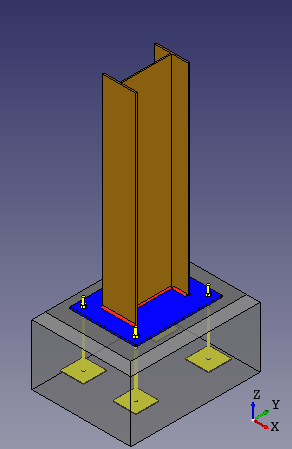
\includegraphics[width=\linewidth]{E:/office _anjali/columnspliceanjali/Osdag3/ResourceFiles/images/3d.png}%
\caption{3D View}%
\end{figure}

%
\end{document}